%% LyX 2.3.4.2 created this file.  For more info, see http://www.lyx.org/.
%% Do not edit unless you really know what you are doing.
\documentclass[english,dvipsnames,aspectratio=169]{beamer}
\usepackage{mathptmx}
\usepackage{eulervm}
\usepackage[T1]{fontenc}
\usepackage[latin9]{inputenc}
\usepackage{babel}
\usepackage{amstext}
\usepackage{amssymb}
\usepackage{graphicx}
\usepackage{ifthen}
\usepackage{xcolor}
\usepackage{xspace}
\usepackage{tikz}
\usetikzlibrary{tikzmark}
\usetikzlibrary{calc}
\usepackage{pgfplots}
%\pgfplotsset{compat=1.17}
\usepackage{booktabs}
\usepackage{xpatch}

\xpatchcmd{\itemize}
  {\def\makelabel}
  {\ifnum\@itemdepth=1\relax
     \setlength\itemsep{2ex}% separation for first level
   \else
     \ifnum\@itemdepth=2\relax
       \setlength\itemsep{1ex}% separation for second level
     \else
       \ifnum\@itemdepth=3\relax
         \setlength\itemsep{0.5ex}% separation for third level
   \fi\fi\fi\def\makelabel
  }
 {}
 {}

\ifx\hypersetup\undefined
  \AtBeginDocument{%
    \hypersetup{unicode=true,pdfusetitle,
 bookmarks=true,bookmarksnumbered=false,bookmarksopen=false,
 breaklinks=false,pdfborder={0 0 0},pdfborderstyle={},backref=false,colorlinks=true,
 allcolors=NYUPurple,urlcolor=LightPurple}
  }
\else
  \hypersetup{unicode=true,pdfusetitle,
 bookmarks=true,bookmarksnumbered=false,bookmarksopen=false,
 breaklinks=false,pdfborder={0 0 0},pdfborderstyle={},backref=false,colorlinks=true,
 allcolors=NYUPurple,urlcolor=LightPurple}
\fi

\makeatletter

%%%%%%%%%%%%%%%%%%%%%%%%%%%%%% LyX specific LaTeX commands.
%% Because html converters don't know tabularnewline
\providecommand{\tabularnewline}{\\}

%%%%%%%%%%%%%%%%%%%%%%%%%%%%%% Textclass specific LaTeX commands.
% this default might be overridden by plain title style
\newcommand\makebeamertitle{\frame{\maketitle}}%
% (ERT) argument for the TOC
\AtBeginDocument{%
  \let\origtableofcontents=\tableofcontents
  \def\tableofcontents{\@ifnextchar[{\origtableofcontents}{\gobbletableofcontents}}
  \def\gobbletableofcontents#1{\origtableofcontents}
}

%%%%%%%%%%%%%%%%%%%%%%%%%%%%%% User specified LaTeX commands.
\usetheme{CambridgeUS} 
\beamertemplatenavigationsymbolsempty


% Set Color ==============================
\definecolor{NYUPurple}{RGB}{87,6,140}
\definecolor{LightPurple}{RGB}{165,11,255}


\setbeamercolor{title}{fg=NYUPurple}
\setbeamercolor{frametitle}{fg=NYUPurple}

\setbeamercolor{background canvas}{fg=NYUPurple, bg=white}
\setbeamercolor{background}{fg=black, bg=NYUPurple}

\setbeamercolor{palette primary}{fg=black, bg=gray!30!white}
\setbeamercolor{palette secondary}{fg=black, bg=gray!20!white}
\setbeamercolor{palette tertiary}{fg=gray!20!white, bg=NYUPurple}

\setbeamertemplate{headline}{}
\setbeamerfont{itemize/enumerate body}{}
\setbeamerfont{itemize/enumerate subbody}{size=\normalsize}

\setbeamercolor{parttitle}{fg=NYUPurple}
\setbeamercolor{sectiontitle}{fg=NYUPurple}
\setbeamercolor{sectionname}{fg=NYUPurple}
\setbeamercolor{section page}{fg=NYUPurple}
%\setbeamercolor{description item}{fg=NYUPurple}
%\setbeamercolor{block title}{fg=NYUPurple}

\setbeamertemplate{blocks}[rounded][shadow=false]
\setbeamercolor{block body}{bg=normal text.bg!90!NYUPurple}
\setbeamercolor{block title}{bg=NYUPurple!30, fg=NYUPurple}



\AtBeginSection[]{
  \begin{frame}
  \vfill
  \centering
\setbeamercolor{section title}{fg=NYUPurple}
 \begin{beamercolorbox}[sep=8pt,center,shadow=true,rounded=true]{title}
    \usebeamerfont{title}\usebeamercolor[fg]{title}\insertsectionhead\par%
  \end{beamercolorbox}
  \vfill
  \end{frame}
}

\makeatother

\setlength{\parskip}{\medskipamount} 

\input ../macros

\begin{document}
\input ../rosenberg-macros

\title[DS-GA 1003]{Statistical Learning Theory\\\vspace{0.5in}\small{Based on David Rosenberg and He He's materials}}
\author{Ravid Shwartz-Ziv}
%{
%    Slides based on Lecture 
%    \href{https://davidrosenberg.github.io/mlcourse/Archive/2019/Lectures/01b.intro-stat-learning-theory.pdf}{1b},
%    \href{https://davidrosenberg.github.io/mlcourse/Archive/2019/Lectures/01c.excess-risk-decomposition.pdf}{1c}
%    from David Rosenberg's \href{https://github.com/davidrosenberg/mlcourse}{course material}.
    
\date{Jan 24, 2023}
\institute{CDS, NYU}

\makebeamertitle
\mode<article>{Just in article version}

\begin{frame}{Decision theory}

\begin{itemize}
\item In data science problems, we generally need to:
\begin{itemize}
    \item<1-> Make a decision:
        \begin{itemize}
            \item Move email to spam folder?
        \end{itemize}
    \item<2-> Take an action:
        \begin{itemize}
            \item In a self-driving car, make a right turn
            \item Reject the hypothesis that $\theta=0$ (classical statistics)
        \end{itemize}
    \item<3-> Produce some output:
        \begin{itemize}
            \item Whose face is it in the image?
            \item The Hindi translation of a Japanese input sentence
        \end{itemize}
    \item<4-> Predicting where a storm will be in an hour (what forms of output are possible here?)
    \item<5-> An \textbf{action} is the generic term for what is produced by our system.
\end{itemize}
\end{itemize}

\end{frame}


\begin{frame}{Inputs}

We make our decision based on context:
\begin{itemize}
\item Inputs {[}ML{]}
\item Covariates {[}Statistics{]}
\begin{exampleblock}{Examples of inputs}
\begin{itemize}
\item A picture
\item The location of the storm in the last 24 hours, other weather-related measurements
\item A search query
\end{itemize}
\end{exampleblock}
\end{itemize}
\end{frame}
%
%\mode<article>{For a search query, the action could be an ordered list of URLs. The
%outcome could be which URL user clicked on first, if any. 
%
%What would be an example of a decision theory problem without an input?
%One off things. e.g. ``guess my number''. You're not producing descision
%function that How about minimizing sum of absolute distance from a
%set of points -- this is called the geometric median. There is no
%closed form expression for the geometric median. You could imagine
%a competition to compute the geometric median for a fixed set of points.
%Each team submits their ``action'', and is evaluated by a loss $\ell(a)=\sum_{i=1}^{n}\left|a-x_{i}\right|$.
%In this class, we'll be able to apply subgradient descent to estimate
%the optimal $a$. {*}{*}{*} But aren't the the points $x_{1},\ldots,x_{n}$
%the ``input''? We could convert this to a problem with input, but
%t hen we have to design a solution for all possible inputs. Perhaps
%we only need to solve the problem once, and the one scenario is special
%case for which we can find the optimal $a$ analytically. }

\begin{frame}{Outcome}

Inputs are often paired with \textbf{outputs} or \textbf{labels}.
\begin{exampleblock}{Examples of outcomes/outputs/labels}
\begin{itemize}
\item Whether or not the picture actually contains an animal
\item The storm's location one hour after they query
\item Which, if any, of the suggested URLs were selected
\end{itemize}
\end{exampleblock}
\end{frame}

\begin{frame}{Evaluation Criterion}

\textbf{Decision theory} is about finding ``optimal'' actions, under
various definitions of optimality.
\begin{exampleblock}{Examples of Evaluation Criteria}
\begin{itemize}
\item Is the classification correct? 
\item Does the transcription exactly match the spoken words?
    \begin{itemize}
        \item Should we give partial credit (for getting only some of the words right)? How?
    \end{itemize}

\item How far is the storm from the predicted location? (If we're producing a point estimate)
\item How likely is the storm's actual location under the predicted distribution? (If we're doing density prediction)
\end{itemize}

\end{exampleblock}
\end{frame}


\begin{frame}{Typical Sequence of Events}

Many problem domains can be formalized as follows:
\begin{enumerate}
\item Observe input $x$.
\item Take action $a$.
\item Observe outcome $y$.
\item Evaluate action in relation to the outcome.
\end{enumerate}

Three spaces:
\begin{itemize}
\item Input space: $\cx$
\item Action space: $\ca$
\item Outcome space: $\cy$
\end{itemize}

\end{frame}

\begin{frame}{Formalization}
\begin{block}{Prediction Function}

A \textbf{prediction function }(or \textbf{decision function}) gets
input $x\in\cx$ and produces an action $a\in\ca$ :

\[
\begin{matrix}f: & \cx & \rightarrow & \ca\\
& x & \mapsto & f(x)
\end{matrix}
\]
\end{block}

\begin{block}<2->{Loss Function}

A \textbf{loss function} evaluates an action in the context of the
outcome $y$.

\[
\begin{matrix}\loss: & \ca\times\cy & \rightarrow & \reals\\
& (a,y) & \mapsto & \loss(a,y)
\end{matrix}
\]
\end{block}
\end{frame}

%\mode<article>{For this course, perhaps the main reason of distinguishing between
%``action space'' $\ca$ and ``outcome space`` $\cy$ is that they
%will be different as soon as next week, when we study classification
%losses. They will be even more different when we study conditional
%probability models, where the action space $\ca$ is probability distributions
%over the outcome space $\cy$. 
%
%Many textbooks, especially more theoretical ones, define loss functions
%as mapping into nonnegative reals, or at least as being bounded below.
%This makes life easier theoretically, since then we know that the
%loss is integrable w.r.t. any probability measure -- i.e. the risk
%is always defined. On the other hand, we want to be able to view maximum
%likelihood estimation in this framework, which uses the ``negative
%log loss'', which is not bounded below. In the Shalev-Shwartz \&
%Ben-David book, they define loss to be nonnegative, but in section
%24.1.2, to tie MLE to ERM, they define a loss function as a negative
%log likelihood. Vapnik, in The Nature of Statistical Learning Theory,
%also has the negative log likelihhood loss.}
%
\begin{frame}{Evaluating a Prediction Function}
    \head{Goal}: Find the optimal prediction function.

    \head{Intuition}: If we can evaluate how good a prediction function is, we can turn this into an optimization problem.

\begin{itemize}
    \item The loss function $\ell$ evaluates a \emph{single} action
    \item How do we evaluate the prediction function \emph{as a whole}?
    \item We will use the standard \textbf{statistical learning theory} framework.
\end{itemize}

\end{frame}


\begin{frame}{Statistical Learning Theory}
Define a space where the prediction function is applicable
\begin{itemize}
\item Assume there is a \textbf{data generating distribution }$P_{\cx\times\cy}.$
\item All input/output pairs $\left(x,y\right)$ are generated i.i.d. from
$P_{\cx\times\cy}.$ 
\end{itemize}

One common desideratum is to have a prediction function $f(x)$ that ``does well on average'':
\[
\ell(f(x),y)\mbox{ is usually small, in some sense}
\]

How can we formalize this?

\end{frame}
\mode<article>{How can we do time series if we require the examples to be iid? Well
- we have think very carefully about these situations. Usually you
try to reframe the inputs (e.g. by featurization) and outputs so they
seem as iid as possible. }

\begin{frame}{Risk}
\begin{definition}
The \textbf{risk} of a prediction function $f:\cx\to\ca$ is
\[
    R(f)=\ex_{(x,y)\sim P_{\cx\times\cy}}\pb{\loss(f(x),y)}.
\]
In words, it's the \textbf{expected loss} of $f$ over $P_{\cx\times\cy}$.
\end{definition}

\begin{alertblock}{We can't actually compute the risk function:}

Since we don't know $P_{\cx\times\cy}$, we cannot compute the expectation.\\
    But we can \textbf{estimate} it.
\end{alertblock}
\end{frame}

\begin{frame}{The Bayes Prediction Function }
\begin{definition}
A \textbf{Bayes prediction function} $\minimizer f:\cx\to\ca$ is
a function that achieves the \emph{minimal risk} among all possible
functions: 
\[
\minimizer f\in\argmin_{f}R(f),
\]
where the minimum is taken over all functions from $\cx$ to $\ca$. 
\end{definition}


\begin{itemize}
\item The risk of a Bayes prediction function is called the \textbf{Bayes
risk}.
\item A Bayes prediction function is often called the ``\textbf{target
function}'', since it's the best prediction function we can possibly
produce.
\end{itemize}
\end{frame}
%
%\begin{frame}{Example: Least Squares Regression}
%\begin{itemize}
%\item Spaces: $\ca=\cy=\reals$
%\item Square loss: 
%\[
%\loss(a,y)=(a-y)^{2}
%\]
%\end{itemize}
%
%\pause{}
%\begin{itemize}
%\item Risk: 
%\begin{eqnarray*}
%R(f) & = & \ex\big[(f(x)-y)^{2}\big]\\
%\pause(\mbox{homework}\implies) & = & \ex\big[(f(x)-\ex[y|x])^{2}\big]+\ex\big[(y-\ex[y|x])^{2}\big]
%\end{eqnarray*}
%\end{itemize}
%
%\pause{}
%\begin{itemize}
%\item So Bayes prediction function is 
%\[
%f^{*}(x)=\ex[y|x]
%\]
%\mode<article>{From the decomposition of expected square error}
%\end{itemize}
%\end{frame}
%%
\begin{frame}{Example: Multiclass Classification}
\begin{itemize}
\item Spaces: $\ca=\cy=\left\{ 1,\ldots,k\right\} $
\item 0-1 loss: 
\[
\loss(a,y)=\ind{a\neq y}:=\begin{cases}
1 & \mbox{if }a\neq y\\
0 & \mbox{otherwise}.
\end{cases}
\]
\end{itemize}

\pause{}
\begin{itemize}
\item Risk: 
\begin{eqnarray*}
R(f) & = & \ex\left[\ind{f(x)\neq y}\right] \quad=0\cdot\pr\left(f(x)=y\right)+1\cdot\pr\left(f(x)\neq y\right)\\
& = & \pr\left(f(x)\neq y\right),
\end{eqnarray*}
which is just the misclassification error rate.

\item The Bayes prediction function returns the most likely
class: 
\[
f^{*}(x)\in\argmax_{1\le c\le k}\pr(y=c\mid x)
\]
\end{itemize}
\end{frame}

\begin{frame}{But we can't compute the risk!}

\begin{itemize}
    \item Can't compute $R(f)=\ex\pb{\loss(f(x),y)}$ because we \textbf{don't know
$P_{\cx\times\cy}$}.

\pause{}
\item One thing we can do in ML/statistics/data science is \textbf{estimate} it:

\pause{}
\begin{block}{Assume we have sample data:}

Let $\cd_{n}=\left((x_{1},y_{1}),\ldots,(x_{n},y_{n})\right)$ be
drawn i.i.d. from $\cp_{\cx\times\cy}$.
\end{block}

\pause{}
\item We draw inspiration from the strong law of large numbers:

If $z_{1},\ldots,z_{n}$ are i.i.d. with expected value $\ex z$,
then
\[
\lim_{n\to\infty}\frac{1}{n}\sum_{i=1}^{n}z_{i}=\ex z,
\]
with probability 1. 
\end{itemize}
\end{frame}

\begin{frame}{The Empirical Risk}

Let $\cd_{n}=\left((x_{1},y_{1}),\ldots,(x_{n},y_{n})\right)$ be
drawn i.i.d. from $\cp_{\cx\times\cy}$.
\begin{definition}
The \textbf{empirical risk}\emph{ }of $f:\cx\to\ca$ with respect
to $\cd_{n}$ is
\[
\hat{R}_{n}(f)=\frac{1}{n}\sum_{i=1}^{n}\loss(f(x_{i}),y_{i}).
\]
\end{definition}

%\begin{itemize}
By the strong law of large numbers, 
\[
\lim_{n\to\infty}\hat{R}_{n}(f)=R(f),
\]
almost surely.


%\item But we want to find the $f$ that \textbf{minimizes} $R(f)$ - will
%minimizing $\hat{R}_{n}(f)$ be good enough?
%\end{itemize}
\end{frame}

\begin{frame}{Empirical Risk Minimization}

\begin{definition}
A function $\hat{f}$ is an \textbf{empirical risk minimizer} if
\[
\hat{f}\in\argmin_{f}\hat{R}_{n}(f),
\]
where the minimum is taken over all functions $f:\cx\to\ca$.
\end{definition}

\begin{itemize}
    \item In an ideal world we'd want to find the risk minimizer.
    \item Is the empirical risk minimizer close enough?
    \item In practice, we always only have a finite sample...
\end{itemize}

\end{frame}

\begin{frame}{Empirical Risk Minimization}

    \begin{itemize}
        \item $P_{\cx}=\mbox{Uniform}[0,1]$, $Y\equiv1$ (i.e. $Y$ is always $1$).

        \item A plot of $\cp_{\cx\times\cy}$:
    \end{itemize}

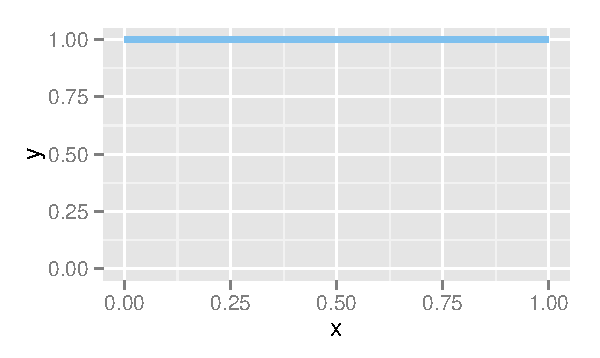
\includegraphics{figures/ERMoverfitting/constantFn} 


\end{frame}

\begin{frame}{Empirical Risk Minimization}

$P_{\cx}=\mbox{Uniform}[0,1]$, $Y\equiv1$ (i.e. $Y$ is always $1$).

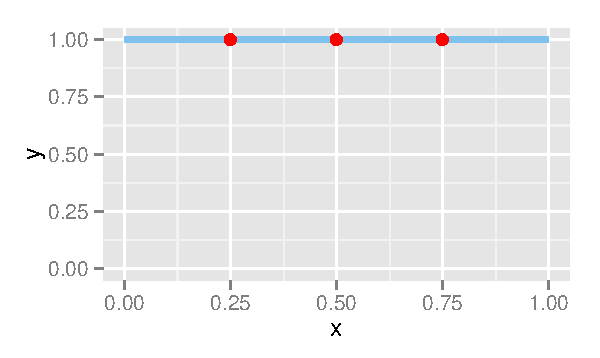
\includegraphics{figures/ERMoverfitting/trainDataConstFn} 

A sample of size $3$ from $\cp_{\cx\times\cy}$.
\end{frame}

\begin{frame}{Empirical Risk Minimization}

$P_{\cx}=\mbox{Uniform}[0,1]$, $Y\equiv1$ (i.e. $Y$ is always $1$).
\begin{center}
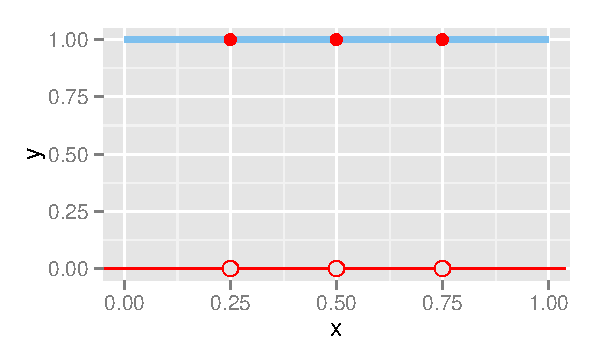
\includegraphics[scale=0.75]{figures/ERMoverfitting/fitAlmostSurely0} 
\par\end{center}

A proposed prediction function:
\[
\hat{f}(x)=\ind{x\in\left\{ 0.25,0.5,0.75\right\} }=\begin{cases}
1 & \mbox{if }x\in\left\{ 0.25,.5,.75\right\} \\
0 & \mbox{otherwise}
\end{cases}
\]

\end{frame}

\begin{frame}{Empirical Risk Minimization}

$P_{\cx}=\mbox{Uniform}[0,1]$, $Y\equiv1$ (i.e. $Y$ is always $1$).

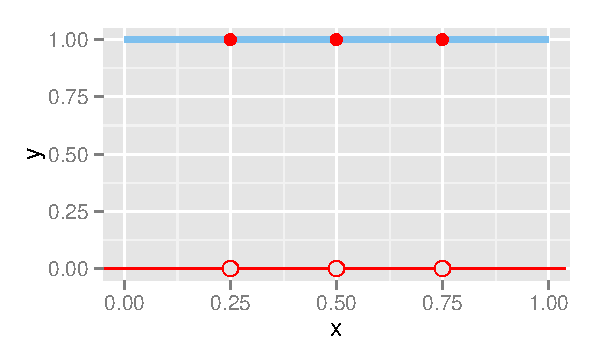
\includegraphics{figures/ERMoverfitting/fitAlmostSurely0} 

Under either the square loss or the 0/1 loss, $\hat{f}$ has Empirical Risk = 0 and
Risk = 1. 
\end{frame}

\begin{frame}{Empirical Risk Minimization}

\begin{itemize}
    \item In this case, ERM led to a function $f$ that just \al{memorized} the data.
\item How can we improve \textbf{generalization} from the training
inputs to new inputs?

\item We need to smooth things out somehow!
\begin{itemize}
\item A lot of modeling is about spreading and extrapolating information
from one part of the input space $\cx$ into unobserved parts of the
space.

\end{itemize}
\item One approach is \textbf{constrained ERM}:

\begin{itemize}
    \item Instead of minimizing empirical risk over \emph{all} prediction functions,
    \item We constrain our search to a particular subset of the space of functions, called a \textbf{hypothesis space}.
\end{itemize}
\end{itemize}
\end{frame}

\begin{frame}{Hypothesis Spaces}
\begin{definition}
A \textbf{hypothesis space} $\cf$ is a set of prediction functions $\cx\to\ca$ that we consider when applying ERM.
\end{definition}

Desirable properties of a hypothesis space:
\begin{itemize}
\item Includes only those functions that have the desired ``regularity'', e.g. smoothness, simplicity
\item Easy to work with (e.g., we have efficient algorithms to find the best function within the space)
\end{itemize}

Most applied work is about designing good hypothesis spaces for specific tasks.
\end{frame}

\begin{frame}{Constrained Empirical Risk Minimization}
\begin{itemize}
\item Given a hypothesis space $\cf$, a set of prediction functions mapping
$\cx\to\ca$,
\item An \textbf{empirical risk minimizer }(ERM) in $\cf$ is a function $\hat{f}_{n}$ such that
\[
    \hat{f}_{n}\in\argmin_{\hl{f\in\cf}}\frac{1}{n}\sum_{i=1}^{n}\loss(f(x_{i}),y_{i}).
\]

\item A \textbf{Risk minimizer }in $\cf$ is a function $\minimizer{f_{\cf}}\in\cf$ such that
\[
    \minimizer{f_{\cf}}\in\argmin_{\hl{f\in\cf}}\ex\pb{\loss(f(x),y)}.
\]
\end{itemize}
\end{frame}

\mode<article>{The hat on $f$ in $\hat{f}_{n}$ indicates that $\hat{f}_{n}$ depends
on the sample data. The subscript $n$ just designates that the sample
was of size $n$.} 

\begin{frame}{Excess Risk Decomposition}
\begin{columns}[c]

\column{.4\textwidth}

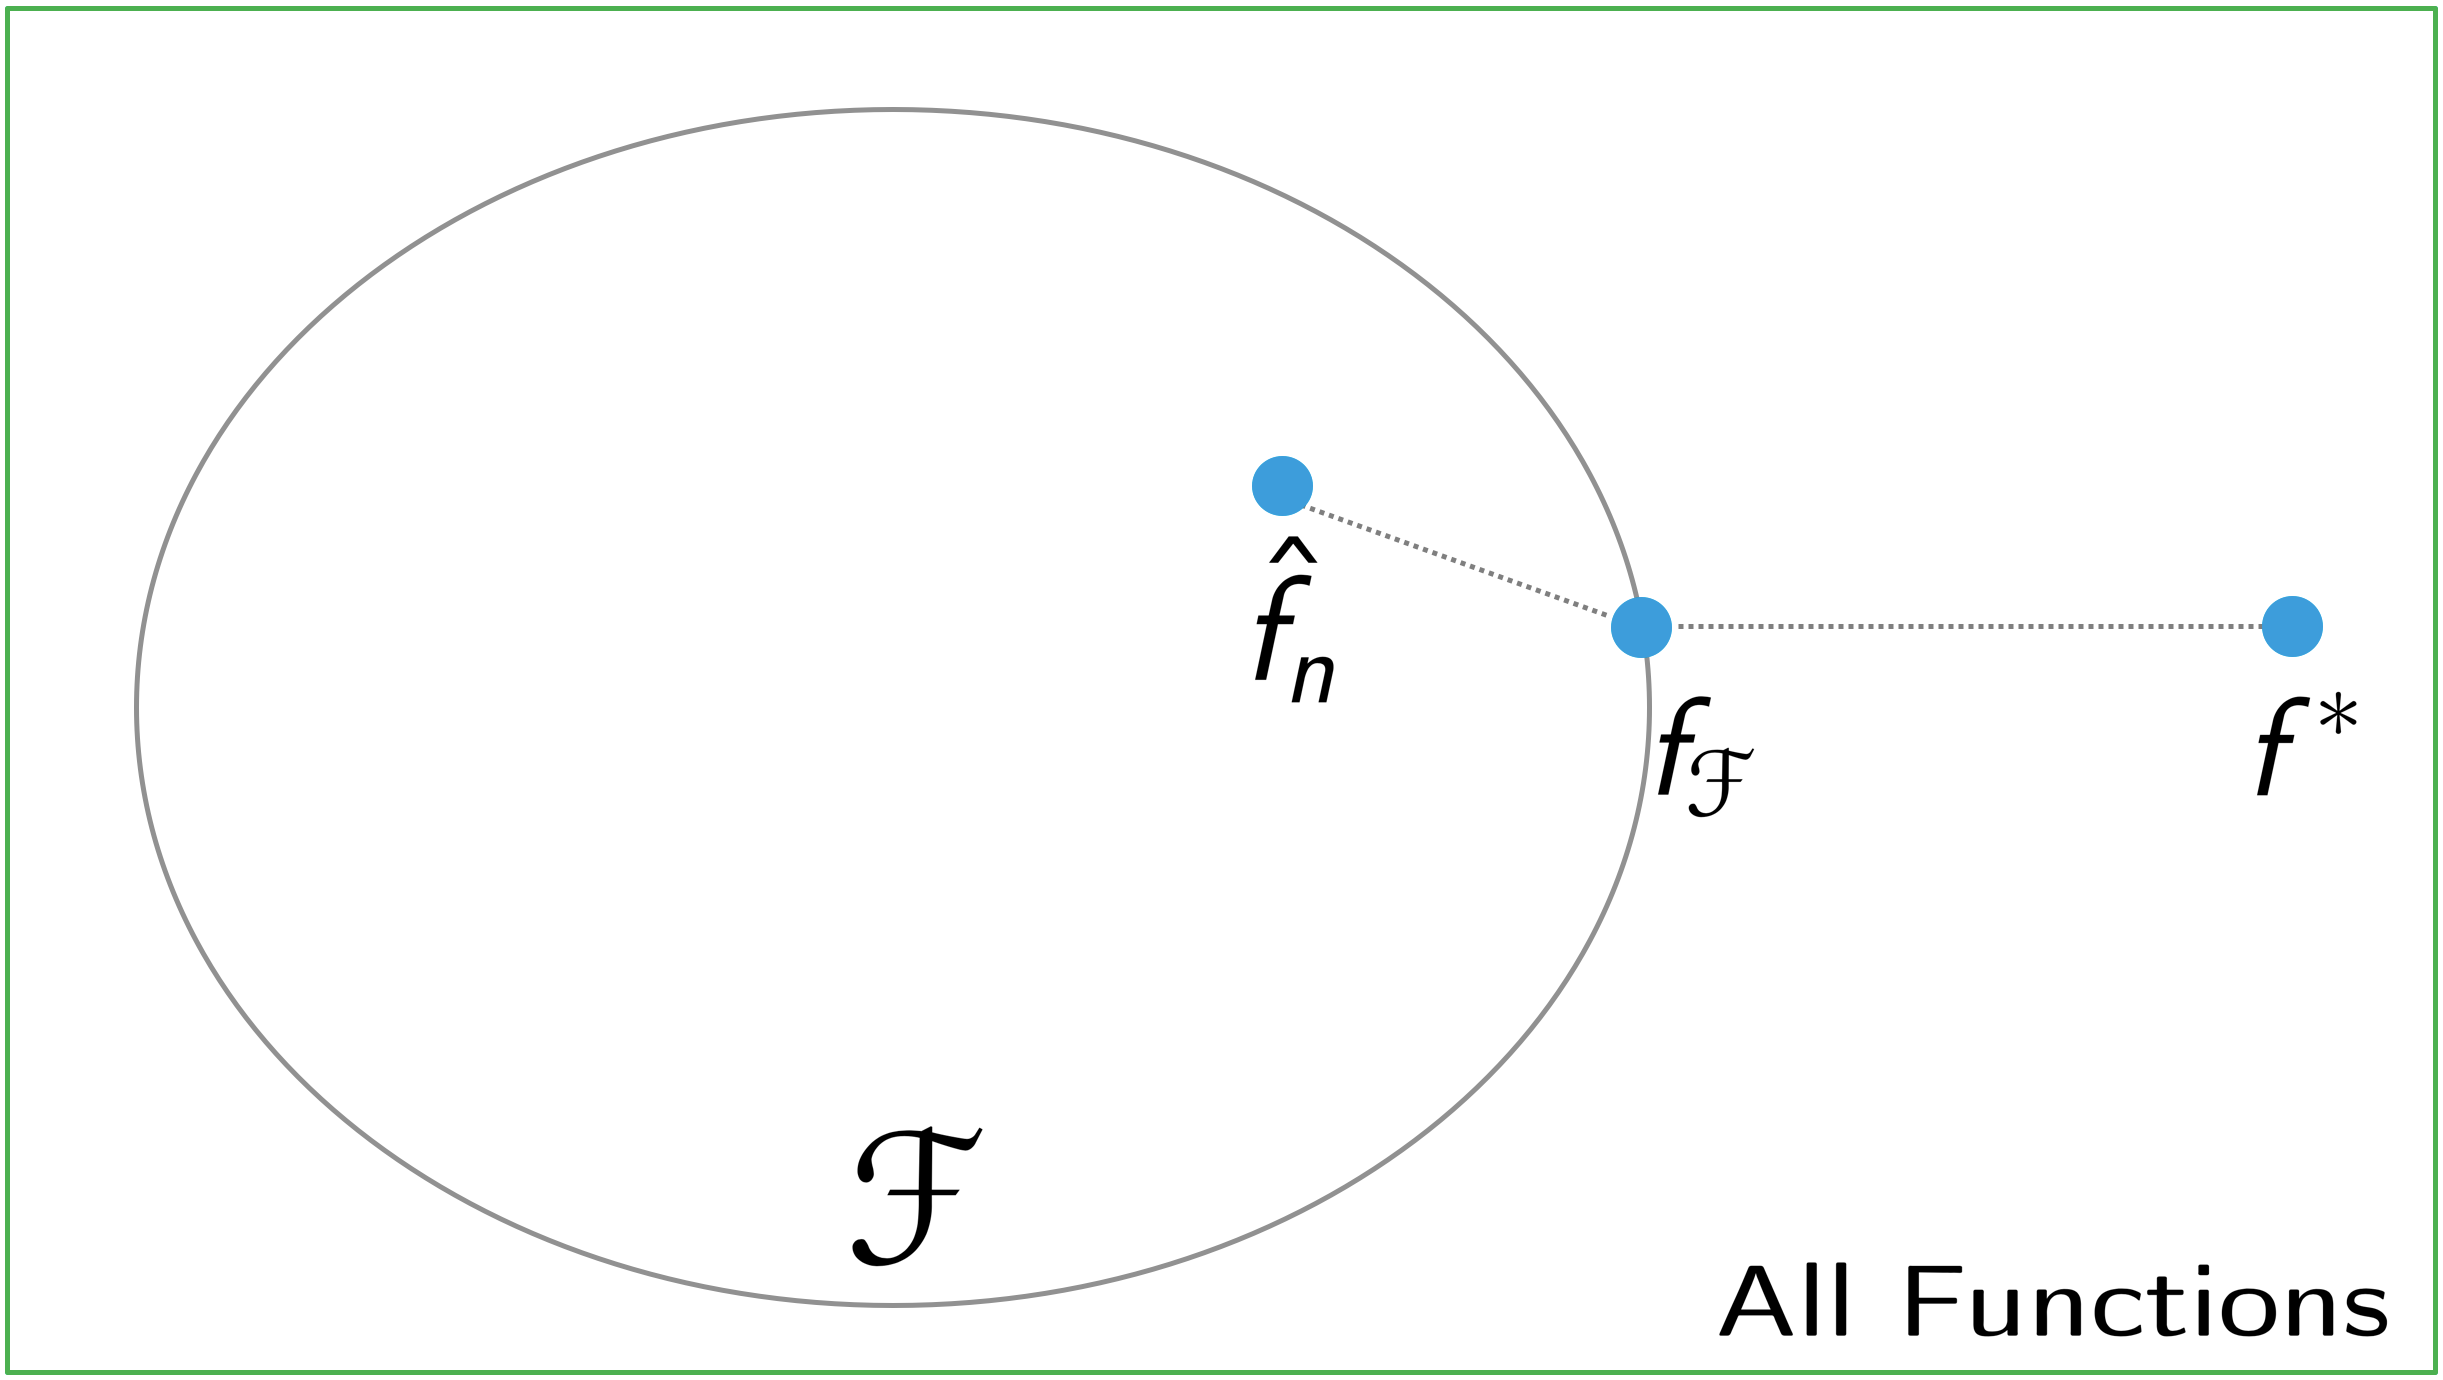
\includegraphics[width=1\columnwidth]{figures/error-decomp}

\column{.4\textwidth}

\begin{align*}
    f^{*}= & \argmin_{f}\ex\pb{\ell(f(x),y)}\\
    f_{\cf}= & \argmin_{f\in\cf}\ex\pb{\ell(f(x),y)}\\
\hat{f}_{n}= & \argmin_{f\in\cf}\frac{1}{n}\sum_{i=1}^{n}\ell(f(x_{i}),y_{i})
\end{align*}
\end{columns}


\begin{itemize}
\item \textbf{Approximation error }(of $\cf$)\textbf{ $=\ R(f_{\cf})-R(\minimizer f)$}
\item \textbf{Estimation error} (of $\hat{f}_{n}$ in $\cf$) $=\ R(\hat{f}_{n})-R(f_{\cf})$ 
\end{itemize}
\end{frame}
\mode<article>{This diagram shows the space of all functions. The hypothesis space
$\cf$ carves out a subset of that space. The Bayes prediction function
$f^{*}$ will not typically be contained in $\cf$. The best we can
possibly do in terms of risk (i.e. the expected loss on a new randomly
chosen data point), which is our ultimate performance measure, is
$f_{\cf}$. How much worse does $f_{\cf}$ perform than $f^{*}$?
That's our potential penalty for restricting to a hypothesis space
$\cf$. We hope it will be more than compensated by reduction in overfitting.
We can write down that performance gap explicitly, and it's called
approximation error. (Parenthetically, Approximation theory is a field
of mathematics that studies how well one can approximate a function
by simpler functions -- e.g. using polynomials, or sins and cosines
or wavelets to approximate a given function. And studying how well
these approximations work.) Approximation error of a hypothesis space
$\cf$ is $\risk(f_{\cf})-\risk(f^{*})$. 

Concept checks: 1) Can approximation error be negative?

2) Is approximation a random quantity?

Now, of course we cannot find $f_{\cf}$, since we can't evaluate
the true risk $\risk$. So in practice, we work with the empirical
risk $\hat{R}$ based on sample of data, a training set. We find the
empirical risk minimizer $\hat{f}_{n}$ in the hypothesis space $\cf$. }

\begin{frame}{Excess Risk Decomposition for ERM}
\begin{definition}
The \textbf{excess risk} compares the risk of $f$ to the Bayes optimal
$f^{*}$:
\[
\mbox{\textbf{Excess Risk}}(f)\,=\,\risk(f)-\risk(\minimizer f)
\]
\end{definition}

\begin{itemize}
\item Can excess risk ever be negative? 
\end{itemize}

The excess risk of the ERM $\hat{f}_{n}$ can be decomposed:
\begin{eqnarray*}
\mbox{\textbf{Excess Risk}}(\hat{f}_{n}) & = & \risk(\hat{f}_{n})-\risk(\minimizer f)\\
& = & \underbrace{\risk(\hat{f}_{n})-\risk(f_{\cf})}_{\text{estimation error}}+\underbrace{\risk(f_{\cf})-\risk(\minimizer f)}_{\text{approximation error}}.
\end{eqnarray*}
\begin{itemize}
\item There is a tradeoff between estimation error and approximation error
\end{itemize}
\end{frame}


\begin{frame}{Approximation Error}

Approximation error $\risk(f_{\cf})-\risk(\minimizer f)$ is
\begin{itemize}
\item a property of the class $\cf$

\item the penalty for restricting to $\cf$ (rather than considering all
possible functions)
\end{itemize}


\emph{Bigger} $\cf$ mean \emph{smaller }approximation error. 

Concept check: Is approximation error a random or non-random variable?
\end{frame}

\begin{frame}{Estimation Error}

Estimation error $\risk(\hat{f}_{n})-\risk(f_{\cf})$
\begin{itemize}
\item is the performance hit for choosing $f$ using finite training data

\item is the performance hit for minimizing empirical risk rather than true
risk 
\end{itemize}

With\emph{ smaller }$\cf$ we expect \emph{smaller }estimation error.

\emph{Under typical conditions: ``}With infinite training data, estimation
error goes to zero.''

Concept check: Is estimation error a random or non-random variable?
\end{frame}

\begin{frame}{ERM in Practice}

\begin{itemize}
\item<1-> What have we been glossing over by writing ``argmin''?

\item<2-> In practice, we need a method to find $\hat{f}_{n}\in\cf$: this can be very difficult!

\item<3-> For nice choices of loss functions and classes $\cf$, we can get
arbitrarily close to the exact minimizer
\begin{itemize}
\item But that takes time -- is it always worth it?
\end{itemize}
\item<4-> For some hypothesis spaces (e.g. neural networks), we don't know how
to find $\hat{f}_{n}\in\cf$. 
\end{itemize}
\end{frame}

\begin{frame}{Optimization Error}
\begin{itemize}
\item In practice, we don't find the ERM $\hat{f}_{n}\in\cf$. 
\item We find $\tilde{f}_{n}\in\cf$ that we hope is good enough.
\item \textbf{Optimization error: }If $\tilde{f}_{n}$ is the function our
optimization method returns, and $\hat{f}_{n}$ is the empirical risk
minimizer, then
\[
\mbox{Optimization Error }=\;R(\tilde{f}_{n})-R(\hat{f}_{n}).
\]
 

%\item Can optimization error be negative? Yes!
%\item But
%\[
%\hat{R}(\tilde{f}_{n})-\hat{R}(\hat{f}_{n})\ge0.
%\]
 
\end{itemize}
\end{frame}

\begin{frame}{Error Decomposition in Practice}
\begin{itemize}
\item Excess risk decomposition for function $\tilde{f}_{n}$ returned by
an optimization algorithm in practice:
\begin{align*}
\mbox{\textbf{Excess Risk}}(\tilde{f}_{n})\, & =\,\risk(\tilde{f}_{n})-\risk(\minimizer f)\\
 & =\underbrace{\risk(\tilde{f}_{n})-R(\hat{f}_{n})}_{\text{optimization error}}+\underbrace{\risk(\hat{f}_{n})-\risk(f_{\cf})}_{\text{estimation error}}+\underbrace{\risk(f_{\cf})-\risk(\minimizer f)}_{\text{approximation error}}
\end{align*}


\item It would be nice to observe the error decomposition for a practical $\tilde{f}_{n}$!
\item How would we address each type of error?
\item Why is this usually impossible?

\item But we could constuct an artificial example, where we know $P_{\cx\times\cy}$
and $f^{*}$ and $f_{\cf}$...
\end{itemize}
\end{frame}

\begin{frame}{ERM Overview}
\begin{itemize}
\item<1-> Given a loss function $\loss:\ca\times\cy\to\reals$,
\item<2-> Choose a hypothesis space $\cf$.
\item<3-> Use an optimization method to find an empirical risk minimizer $\hat{f}_{n}\in\cf$:
\[
\hat{f}_{n}=\argmin_{f\in\cf}\frac{1}{n}\sum_{i=1}^{n}\loss(f(x_{i}),y_{i}).
\]
\item<4-> (Or find a $\tilde{f}_{n}$ that comes close to $\hat{f}_{n}$)
\item<5-> The data scientist's job: 
\begin{itemize}
\item Choose $\cf$ that balances approximation and estimation error.
\item As we get more training data, we can use a bigger $\cf$.
\end{itemize}
\end{itemize}
\end{frame}

\end{document}
